\chapter{Approach and Results}\label{chap:chap4}


This chapter presents the main work which derived from the study performed in Chapter~\ref{chap:sota}.


MUST COMPLETE INTRO


\section{Implementation}\label{sec:implementation}


\subsection{Web system}

Two frameworks were considered for building the web system:

\begin{enumerate}
\item Ruby on Rails;
\item Django.
\end{enumerate}

As it was concluded in Chapter~\ref{chap:sota} --~\nameref{chap:sota} -- in the section~\nameref{sota:concl}, \textit{Django} (and consequently \textit{Python}) was chosen for the development of the web system.

Some of the functionalities implemented are documented in the next part of this chapter.

\subsubsection{Web system functionalities}

In this segment of the document, some of the web system functionalities are document with regards to their technical aspect.\\
\ \\
\textbf{The login system}:\\
\ \\
The login system was implemented using the \texttt{django.contrib.auth} module (referred to as: ``Authentication module'' for the rest of the chapter for readability reasons) which comes bundled with a clean \textit{Django} installation.

This module automates the process of managing users, permissions and the overall authentication aspect of a system, by providing a pre-created ``Model'' with a set of attributes,  (\textit{Django} uses an MVC architecture, as mentioned in Chapter~\ref{chap:sota} --~\nameref{chap:sota}, section~\nameref{inserir seccao do sota onde o django e comentado}) which can be edited if the necessity arises.

This module handles every user as a ``normal'' user unless the fields ``is\_staff'' and/or ``is\_superuser'' are changed to ``True'' (these fields are present ), which mean that a user will be able to access the administration panel and have all the permissions inside the system without needing to explicitly assigning them, respectively.

In the context of this project, the system administrator is a ``superuser'' and is the only one who can access the administration panel. If there is a need of creating extra administrators, it can be easily done by accessing the administration panel and following the instructions displayed.

In order to know which user has access to what, the user who is currently logged in is saved in the current session. As such, it is possible to know which user is currently accessing the viewed page (by accessing \texttt{request.user} in the \textit{Django} ``view'' for the current page) and take actions accordingly. In this project, if a user is not logged in, he/she cannot access the system at all, being redirected to a login page each time they try and fail. 

The administrator is shown a link to ``Management'' section hidden in the ``Index'' page from the rest of the users, using the same login system. The ``view'' checks if the current user has the field ``is\_staff'' set to ``True'' and if it is, that link is shown.

Even if the normal users are aware of the management area and know the link to it, they still cannot access it even if they are logged in, since the ``view'' for that page checks if the user has access, thus preventing an outsider from doing harm to the system.\\
\ \\
\textbf{The ``Search'' function and the ``Tag'' system}:\\
\ \\
In order to provide for a better VM image management, it was decided to implement a search function, where users could easily find which VM images they were looking for with little effort required. 

The search function itself is not hard to implement, as long as the fields it searches over are properly created. As such, it was necessary to identify which fields would be used.

\textit{Django} has a module that covers that necessity. This module (called \texttt{django-tagging}), allows for the association of a number of ``tags'' with any instance of any ``Model'' and simplifies the process of working with ``tags''~\cite{django-tagging}. Upon the discovery of this module, attempts of working with either the ``Image name'' or the ``Image description'' fields were automatically discarded.

The user has the ability of ``tagging'' an image on its creation process simply by typing which keywords he/she wishes to attach to that image. Multiple word keywords are supported, as long as they are separated via commas (specified in the image creation page).

This ``tag'' system now allows for the search function to use them. When the user uses this function, he/she has to type in which keywords to search for. The system will then iterate over the tags which were inputted and search in the system for all the images which were tagged with that keyword, using a method included in the \texttt{django-tagging} module called \texttt{get_by_model} which takes the ``Model'' that is needed to search over and the keyword inputted in the search form.

The ``Search'' function also updates the frequency of which the ``tags'' were searched. If the search term does not exist in the database, it is created with the usage of ``1''. If it exists, its usage is incremented once.\\
\ \\
\textbf{Helping the user choose a VM image}:\\
\ \\
As it was mentioned in Chapter~\ref{chap:chap4} --~\nameref{chap:chap4}, in section~\nameref{seccao onde se fala da ajuda que se da ao utilizador} -- different types of ``tools'' were implemented in order to help the user choose which VM he/she should use:

\begin{itemize}
\item A set of statistics;
\item A search function.
\end{itemize}

\ \\
The set of statistics contains the following:

\begin{enumerate}
\item What VM images the user that is logged in has available to him (this includes public images and those the user created);
\item Which VM images are more used across the system;
\item Which ``tags'' were most searched across the system;
\item A ``Tag'' Cloud was created, showing which ``tags'' were most used across the system.
\end{enumerate}
\ \\
These statistics were implemented by taking advantage of the relationships created and depicted in the UML diagram shown in the previous section (~\nameref{seccao onde esta o diagrama uml}). 

As it can be understood from the diagram, there is a direct relation between the user and the VM image, as an image has an owner explicitly declared in its attributes.

Combining the knowledge from the current user in section (explained earlier in this chapter) and that relation, collecting which VM images the user has created becomes relatively easy. After this, all that is needed to do is collect which VM images are marked as being public and display the two lists combined. The possibility of having a duplicate image is possible (since one of the users images may be set as public) is addressed and is prevented by checking if any of the elements from the first list already exists in the second list.

As for knowing which VMs are more used across the system, this is done by using association derived from the relationship between images and users (represented as ``Usage'' in the UML diagram). Each time a VM image is launched, the system internally increases the number of uses from that image by taking the elements that identify the VM image and the user in session. 

As it was explained earlier, when the user search for a ``tag'', the number of uses of that ``tag'' increases internally.

The creation of a ``Tag'' cloud is also a built-in functionality of the \texttt{django-tagging} module. What it does it create a list of the ``tags'' used for a specified ``Model'', using how many times the ``tags'' were used and associate them with a certain font size to be displayed. This assignment uses either a logarithmic or a linear distribution so that a visual comparison can be made. The bigger the used font, the more times that tag was used~\cite{http://django-tagging.googlecode.com/svn/trunk/docs/overview.txt}.\\
\ \\
\textbf{VM image creation}:\\
\ \\
The VM image creation was created by using \texttt{bash}~\footnote{Unix command shell.} scripts. The web system calls these scripts and they are ran server side. An example of those scripts can be found in Appendix~\ref{ap:ap4} (~\nameref{ap:ap4}).

These scripts are created using the information inputted by the user in the VM image creation page. They take the name of the image and the name of the programs to be included in the VM creation in order to contextualize it. 

These scripts are built using \textit{Python}'s ability to write to file and they are stored server side. The files must be opened using the arguments ``r+'', which means that the script will be overwritten every time a VM image is created.

In order for the scripts to be run, whichever user is logged into the server and runs the web system needs to have specific passwordless "Superuser" (\texttt{sudo}) access to that script. This needs to be done since \texttt{vmbuilder} requires \texttt{sudo} permissions. 

This access can be granted by modifying the \texttt{sudoers} file and granting \texttt{sudo} permission to the user which will run the web system and \emph{only} to the files which need to be run.

This guarantees that nothing in the system is compromised and that only specific scripts can be ran using \texttt{sudo} permissions.\\
\ \\
\textbf{Managing tasks}:

falar do celery


insert this script somewhere 

One thing to have in mind is that the VM image creation process is very time consuming. Several tests were ran and the average time passed the twenty minute timeframe, on a small deployment (only \texttt{vim} and \texttt{openssh-server} were downloaded and installed). One of the script executions can be seen in Figure~\ref{fig:script-timer}.

\begin{figure}[h]
  \begin{center}
    \leavevmode
    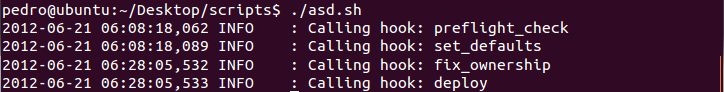
\includegraphics[width=\linewidth]{script-timer}
    \caption{One of the VM image creation test runs.}
    \label{fig:script-timer}
  \end{center}
\end{figure}


----- derpderpderp

The modules \texttt{python-tagging} and \texttt{South} are needed for the web application to function properly. \texttt{python-tagging}, as it was mentioned earlier, is crucial for the search function, whereas \texttt{South} is used in database migrations.


\pagebreak











\section{Integrating with OpenStack}

Connection with \textit{Glance} is made through a RESTful API. Communication with \textit{Glance} is established when the user wants to store a newly created VM image, wishes to use an already existing one and when the user wishes to view the images already stored in the server. This last case can be eliminated by storing the previous results on a text file, along with the timestamp of the last change made to that list (which should happen when a user creates and inserts a new VM image into the system).

Since the web application has \textit{Python} code on the background and \textit{OpenStack} is coded in the same programming language, this connection is seamless.
%The application of the design and architecture described in Chapter~\ref{chap:chap3} is presented, being divided in three main areas:

%\begin{itemize}
%\item Cloud environment deployment (\textit{OpenStack});
%\item Development of a web application;
%\item Creation and management of VM images (communication between the two parts of the system mentioned in the previous bullet points).
%\end{itemize}

\subsection{Cloud environment deployment}\label{subsec:cloud_env}

As mentioned in Chapter~\ref{chap:sota}, section~\ref{subsubsec:devstack}, \textit{DevStack} was used in order to simplify the cloud deployment.

Firstly, a clean installation of Ubuntu 12.04 LTS (as recommended by \textit{DevStack}' homepage) was created on Linux's \textit{Virtual Machine Manager} (\textit{libvirt}).

\textit{DevStack} deployment instructions were followed as they are in its webpage~\footnote{\url{http://devstack.org}} and after the script finished, the \textit{Horizon} Dashboard was accessible via a webpage, as it can be seen in Figure~\ref{fig:stack-dashboard}.

\begin{figure}[t]
  \begin{center}
    \leavevmode
    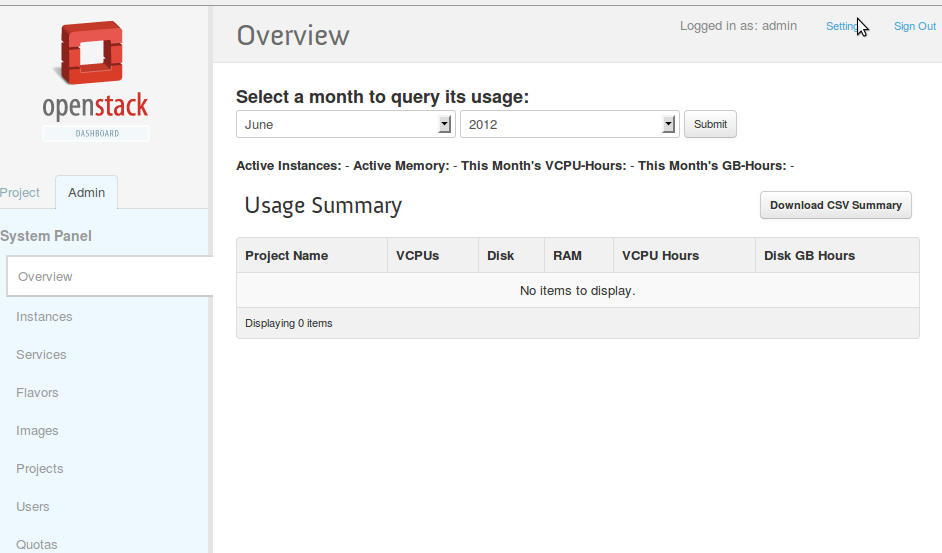
\includegraphics[width=\linewidth]{dashboard}
    \caption{\textit{OpenStack Horizon} Dashboard.}
    \label{fig:stack-dashboard}
  \end{center}
\end{figure}

All the desired services were up and running, as shown in Figure~\ref{fig:services}. Even though the image service (\textit{Glance}) was what was needed the most, it showed that the \textit{DevStack} deployment is a viable \textit{OpenStack} development tool.

\begin{figure}[h]
  \begin{center}
    \leavevmode
    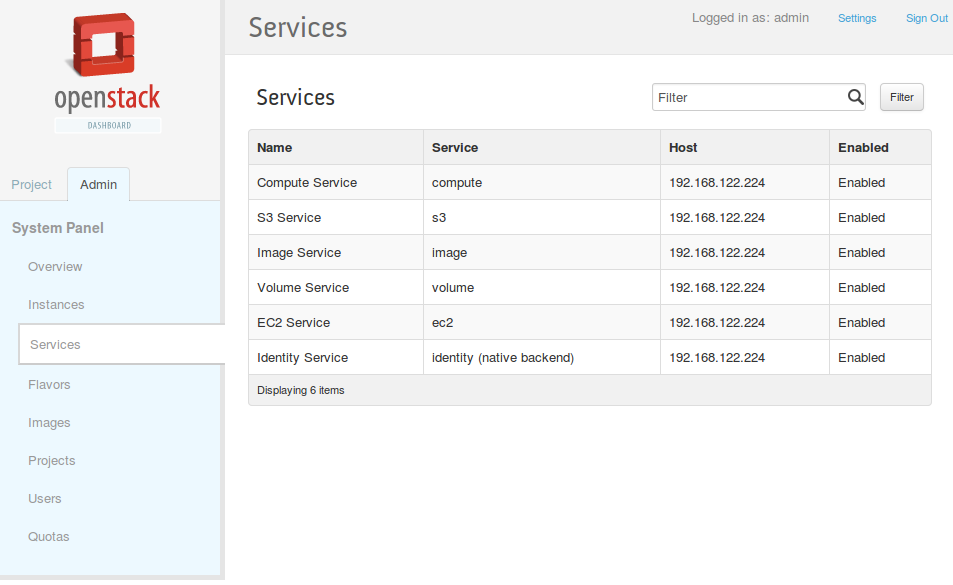
\includegraphics[width=\linewidth]{services}
    \caption{\textit{OpenStack} services.}
    \label{fig:services}
  \end{center}
\end{figure}

%\subsection{Creation and management of VM images}\label{subsec:vm-create-manage}

%As it was concluded in Chapter~\ref{chap:chap3} (~\nameref{chap:chap3}), the VM creation was implemented by using \textit{Ubuntu}'s \texttt{vmbuilder}. 

%A \texttt{bash} script was created in order to automate the process. Since it is nothing more than a text file, it is easily modified by the \textit{Python} classes which are called by the web application. The user needs ``write'' permissions to run that file. An example of the script is attached in Appendix~\ref{chap:ap4} -~\nameref{chap:ap4}.

%This script is run when the user finishes the VM image creating process in the web application.


The modules \texttt{python-tagging} and \texttt{South} are needed for the web application to function properly. \texttt{python-tagging}, as it was mentioned earlier, is crucial for the search function, whereas \texttt{South} is used in database migrations.


\clearpage
\subsection{Connecting the dots}\label{subsec:architecture}

As mentioned in Chapter~\ref{chap:sota}, section~\ref{subsec:openstack}, \textit{OpenStack} is designed to deliver a massively scalable cloud operating system, each of the components being designed to work together in order to prodive complete IaaS. This integration is facilitated through pulic APIs that each service offers, being available to the cloud's end users.~\cite{ken-pepple:essex-arch}. 

Expanding the diagram shown in Figure~\ref{fig:openstack_sw_diag}, the relationships between the services are shown in Figure~\ref{fig:openstack_services}:

\begin{figure}[h!]
  \begin{center}
    \leavevmode
    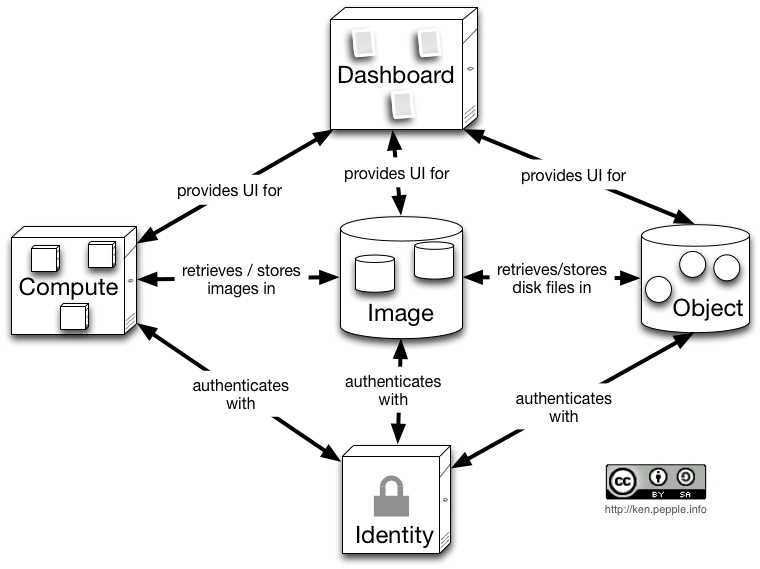
\includegraphics[scale=0.5]{nova-concept-int-essex}
    \caption{Relationships between the different \textit{OpenStack} services.~\cite{ken-pepple:essex-arch}}
    \label{fig:openstack_services}
  \end{center}
\end{figure}

The solution proposed for this project links the \textit{OpenStack} Dashboard --- \textit{Horizon} --- with the designed \textit{Web application} developed in \textit{Python} and \textit{Django}, as shown in Figure~\ref{fig:architecture}.

\begin{figure}[t]
  \begin{center}
    \leavevmode
    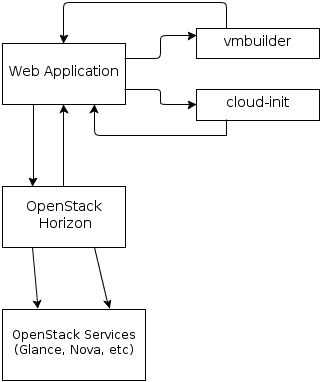
\includegraphics[scale=0.5]{architecture}
    \caption{Proposed architecture implementation.}
    \label{fig:architecture}
  \end{center}
\end{figure}

As it can be observed, the web application will use \texttt{vmbuilder} and \textit{cloudinit} whenever needed and then passing that information to the \textit{OpenStack Horizon} dashboard, which will communicate with the rest of \textit{OpenStack} services.

Since \texttt{vmbuilder} and \textit{cloudinit} work for different purposes (\texttt{vmbuilder} creates contextualized VM images and \textit{cloudinit} contextualizes clean VM images), different tools will be used for different purposes.



An interesting feature to complete in future work could be eliminating the web system and passing the image creation and contextualization to \textit{OpenStack}, modifying the \textit{Horizon} dashboard itself.
 

\section{Conclusions}

This chapter presented how the architecture described in the previous chapter (\nameref{chap:chap3}) was implemented, as well as what were the use cases, the challenges encountered and if and how they were overcome. 
As for the goal completion, \textit{OpenStack} was fully deployed, as well as the web application. VM image creation was successful, as well as the contextualization process.


MUST COMPLETE CONCLUSIONS
